\section{First strategy}

Alice determines a sequence of vertices of the graph $G$ satisfying $col_{2}(G)$. The game begins only after.

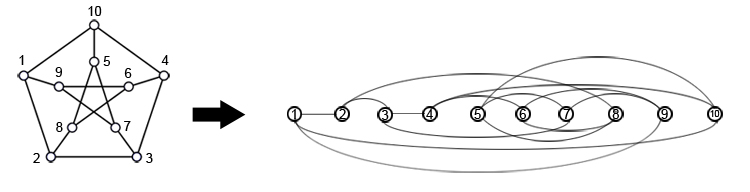
\includegraphics[width=13cm]{IntroOrder.jpg}
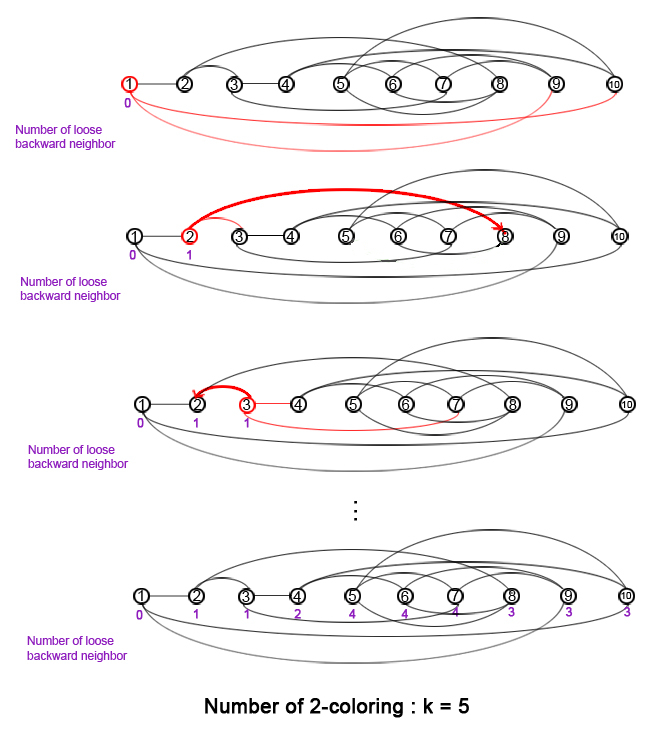
\includegraphics[width=10cm]{orderstep.jpg}

When Bob colors a vertex $v_{h}$,
Alice's strategy is to seek in the order previously determined the loose backward neigbor of $v_{h}$ not yet
colored having the lowest index. Once found, it is colored. If Alice does not find such a vertex, she simply picks from the uncolored vertices set the one with the lowest index in the order.
According to this strategy, each graph $G$ satisfies $\chi_{g}(G) \leq \chi(G) \times (1 + col_{2}(G))$.

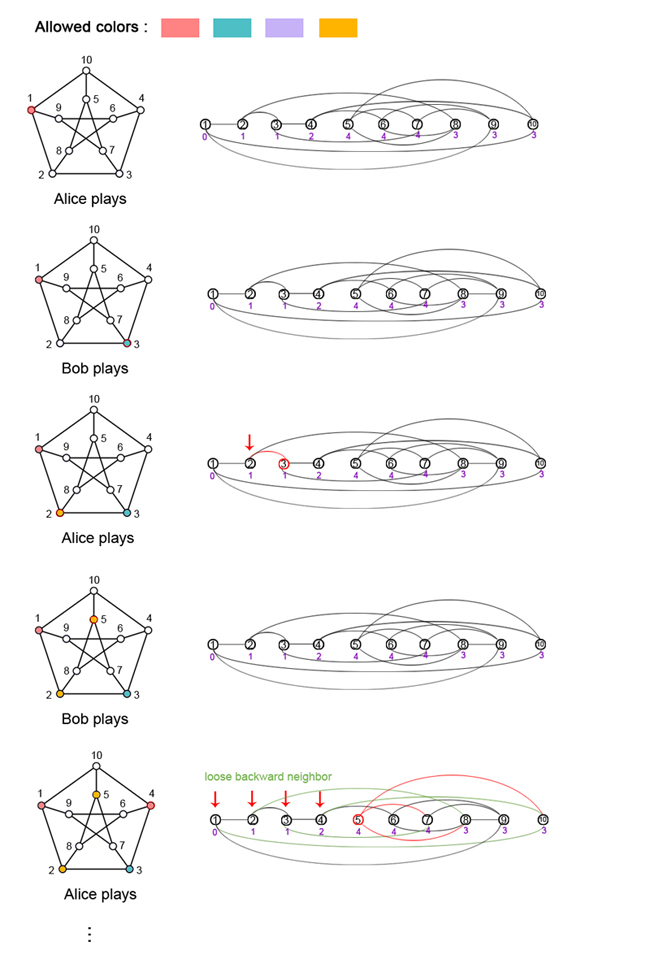
\includegraphics[width=13cm]{gameS1.jpg}